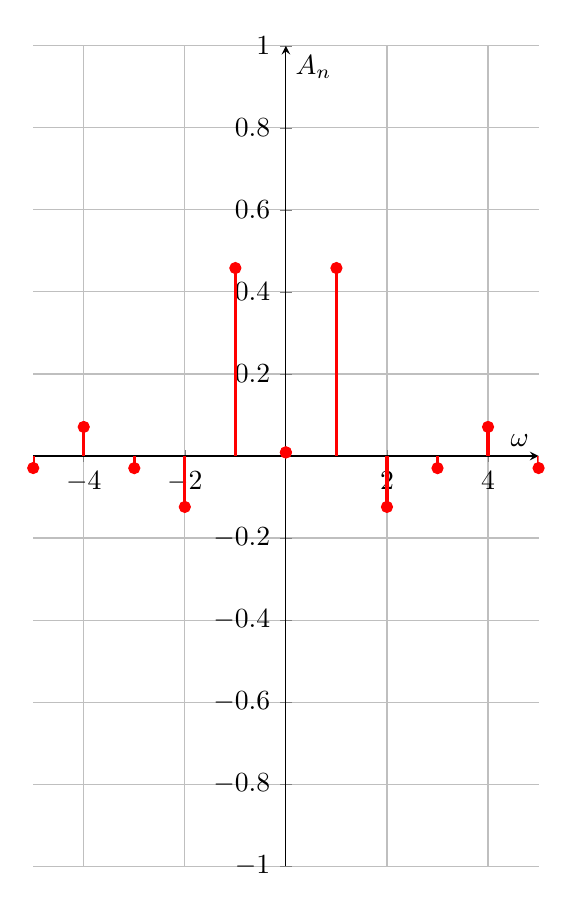
\begin{tikzpicture}
	\begin{axis}[axis lines=middle, grid=both, height=12cm, width=8cm, xmin=-5, xmax=5, ymin=-1, ymax=1, xlabel = $\omega$, ylabel = $A_n$]
		\foreach \x in {0,...,5}{
			\addplot[mark=none, red, very thick] coordinates { (\x, 0) ({\x}, {0.5 * 1/(2 * \x - 1) * sin(2 * deg(\x) - 1)}) };
			\addplot[mark=none, red, very thick] coordinates { (-\x, 0) ({-\x}, {0.5 * 1/(2 * \x - 1) * sin(2 * deg(\x) - 1)}) };
			\addplot[only marks, red] coordinates{ (\x, {0.5 * 1/(2 * \x - 1) * sin(2 * deg(\x) - 1)}) };
			\addplot[only marks, red] coordinates{ (-\x, {0.5 * 1/(2 * \x - 1) * sin(2 * deg(\x) - 1)}) };
		}
	\end{axis}
\end{tikzpicture}